Neste capítulo apresentamos o algoritmo \algname{Poset Forest Search} 
(\algname{PFS}), um algoritmo ótimo para o problema U-Curve que foi 
criado para enfrentar a limitação do algoritmo \algname{U-Curve Branch 
and Bound} (\algname{UBB}) ser unidirecional. Apesar do \algname{PFS}
ter solucionado tal problema com sucesso, este algoritmo apresenta 
pontos que ainda podem ser explorados para se criar uma modificação que
tenha melhor desempenho computacional. Modificaremos então o 
\algname{PFS}, explorando tais pontos.

Baseamos nosso trabalho no código já feito por Reis, que é software 
livre e está disponível no arcabouço \toolname{featsel} \cite{Reis+17} 
sob a licença de uso \foreignword{GNU General Public License}.

\section{Descrição do algoritmo}
% - apresentar o UBB
%   - organização do espaço de busca em uma árvore
%   - pilha de busca em profundidade -> simples poda: não inserir nó
%     na pilha 
%   - limitação por ser unidirecional
% - apresentar o PFS
%   - duas florestas
%     - é bom explicar o que é leftmost aqui
%   - regras do jogo
%   - pseudo-código com as duas etapas
%   - indicar quais são os pontos que podem ser explorados

\subsection{O caso simples: \algname{U-Curve Branch and Bound}}
O algoritmo \algname{U-Curve Branch and Bound} (\algname{UBB}), que é 
uma versão simplificada do \algname{PFS}, percorre o espaço de busca 
fazendo uma busca em profundidade em uma árvore que é subgrafo do 
diagrama de Hasse do reticulado Booleano ($\powerset (S), \subseteq$). 
Esta árvore é definida por aplicações recursivas do seguinte lema:

\begin{mylemma}
\label{lemma:lower_forest}
Sejam $X$ e $Y$ conjuntos, $X$ não-vazio e $x_i$ o $i$-ésimo 
elemento de $X$. Seja $X_0 \supseteq X_1 \supseteq \dots \supseteq 
X_{|X|}$ uma cadeia tal que $X_0 = X$, $X_{|X|} = \emptyset$ e $X_{i} 
\cup \{x_i\} = X_{i - 1}$ para todo $0 < i \leq |X|$. Vale que:
\begin{align*}
\{ Y \} \cup \bigcup_{i = 1}^{|X|} \{W \cup Y \cup \{x_i\} : W \in \powerset (X_i)\} = \{W \cup Y : W \in \powerset (X)\}.
\end{align*}
\end{mylemma} 

\begin{proof}
Faremos uma prova por indução no tamanho de $X$ de maneira similar a
Reis ~\cite{Rei12}.

\begin{itemize}
\item{Suponha que $|X| = 1$. Então:}
\begin{align*}
    \{Y\} \cup \bigcup_{i = 1}^{1} \{W \cup Y \cup \{x_i\} : W \in \powerset (X_i)\} & = 
    \{Y\} \cup \{W \cup Y \cup \{x_1\} : W \in \powerset (X_1)\} & \\
    & = \{Y\} \cup \{Y \cup \{x_1\}\} \tag{Como $X_1 = \emptyset$} \\
    & = \{Y, Y \cup \{x_1\}\} \\
    & = \{W \cup Y : W \in \powerset (X)\}
\end{align*}

\item{Suponha que o lema é verdadeiro para todo $X$ com $|X| < k$, 
    então:}
\begin{align*}
    & \{Y\} \cup \bigcup_{i = 1}^{k} \{W \cup Y \cup \{x_i\} : W \in \powerset (X_i)\} = \\
    & \{Y\} \cup \bigcup_{i = 2}^{k} \{W \cup Y \cup \{x_i\} : W \in \powerset (X_i)\} \cup \{W \cup Y \cup \{x_1\} : W \in \powerset (X_1) \}\\
\end{align*}
Seja $Z = Z_0 = X_1, Z_1 = X_2, \dots Z_{|Z|} = X_{|X|}$, então
$|Z| = k - 1$ e $z_1 = x_2, z_2 = x_3, \dots, z_{|Z|} = x_{|X|}$, e
\end{itemize}

\begin{align*}
    & \{Y\} \cup \bigcup_{i = 2}^{k} \{W \cup Y \cup \{x_i\} : W \in \powerset (X_i)\} \cup \{W \cup Y \cup \{x_1\} : W \in \powerset (X_1) \} =\\
    & \{Y\} \cup \bigcup_{j = 1}^{k - 1} \{W \cup Y \cup \{z_j\} : W \in \powerset (Z_i)\} \cup \{W \cup Y \cup \{x_1\} : W \in \powerset (X_1) \} =\\
    \tag{Pela hipótese de indução}  \\ 
    & \{Y \cup W : W \in \powerset (Z)\} \cup \{W \cup Y \cup \{x_1\} : W \in \powerset (X_1) \} =  \\
    & \{Y \cup W : W \in \powerset (X_1)\} \cup \{W \cup Y \cup \{x_1\} : W \in \powerset (X_1) \} =  \\
    & \{Y \cup W : W \in \powerset (X_1 \cup {x_1})\} = \\
    & \{Y \cup W : W \in \powerset (X)\} \\
\end{align*}
\end{proof}

Para representar o espaço de busca como uma árvore, devemos aplicar o
lema da seguinte forma. Vamos utilizar o conjunto $X_Y$ para determinar 
para cada nó $Y$ do reticulado quais são os nós alcançáveis por ele, de
maneira que um nó $Y$ pode alcançar todo nó do intervalo 
$[Y, X_Y \cup Y]$. Iniciamos a construção da árvore com a base da 
aplicação recursiva do lema, indicando que $X_{Y = \emptyset} = S$, 
pois $\emptyset$ deve ser a raiz da árvore e deve alcançar qualquer 
outro nó. Agora suponha que estamos em um nó $Y$, então
definimos $X_0 = X_Y$, $X_{Y_i} \cup \{x_i\} = X_{Y_{i - 1}}$, e 
$Y_i = Y \cup \{x_i\}$ para $x_i \in X_Y$; então para criar a sub-árvore 
com raiz $Y$ basta adicionar os arcos $(Y, Y_i)$ para cada $i$ e aplicar 
o lema recursivamente para cada $Y_i$ e $X_{Y_i}$. A figura 
~\ref{fig:pfs:ubb_tree} mostra uma árvore arbitrária gerada pela 
aplicação recursiva do lema. 

\begin{figure}[!ht]
  \centering 
  \begin{tabular}{c c}
    \subfigure[] {\scalebox{0.4}{
     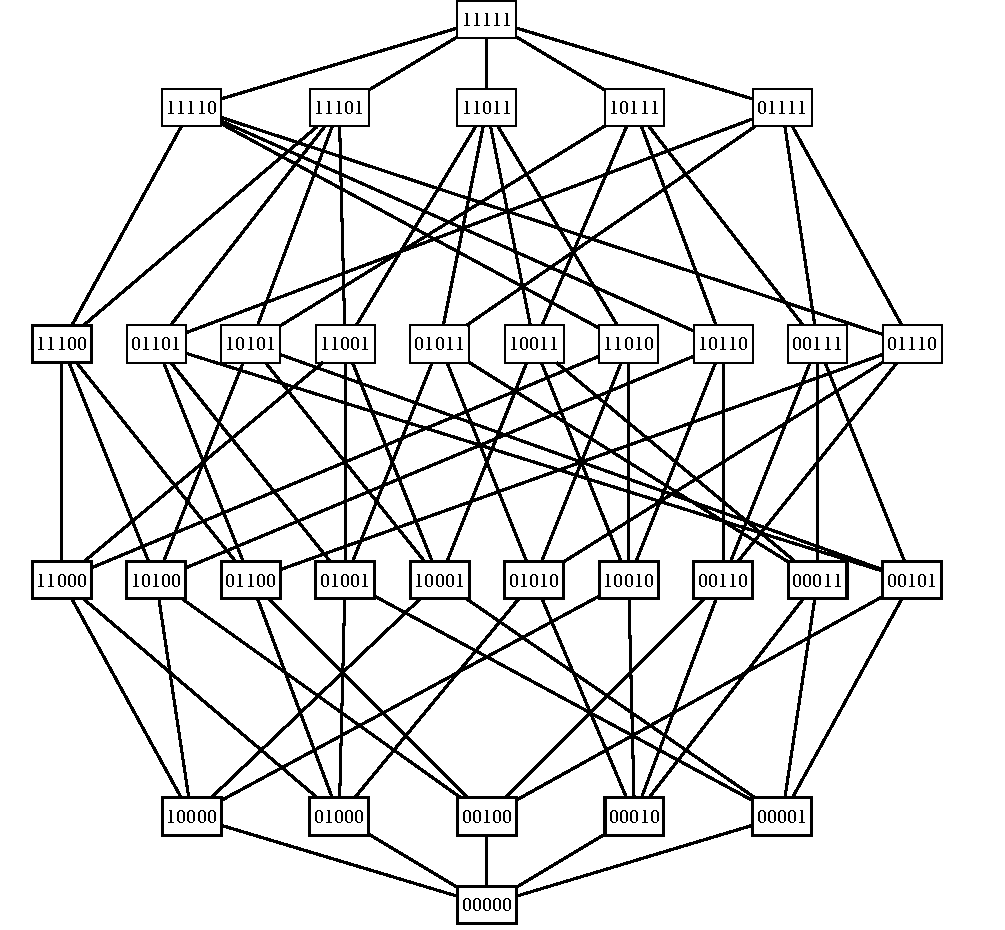
\includegraphics[clip=true]{pfs/ubb/full_lattice.pdf}}
     \label{fig:ubb:full} }
    & 
    \subfigure[] {\scalebox{.4}{
    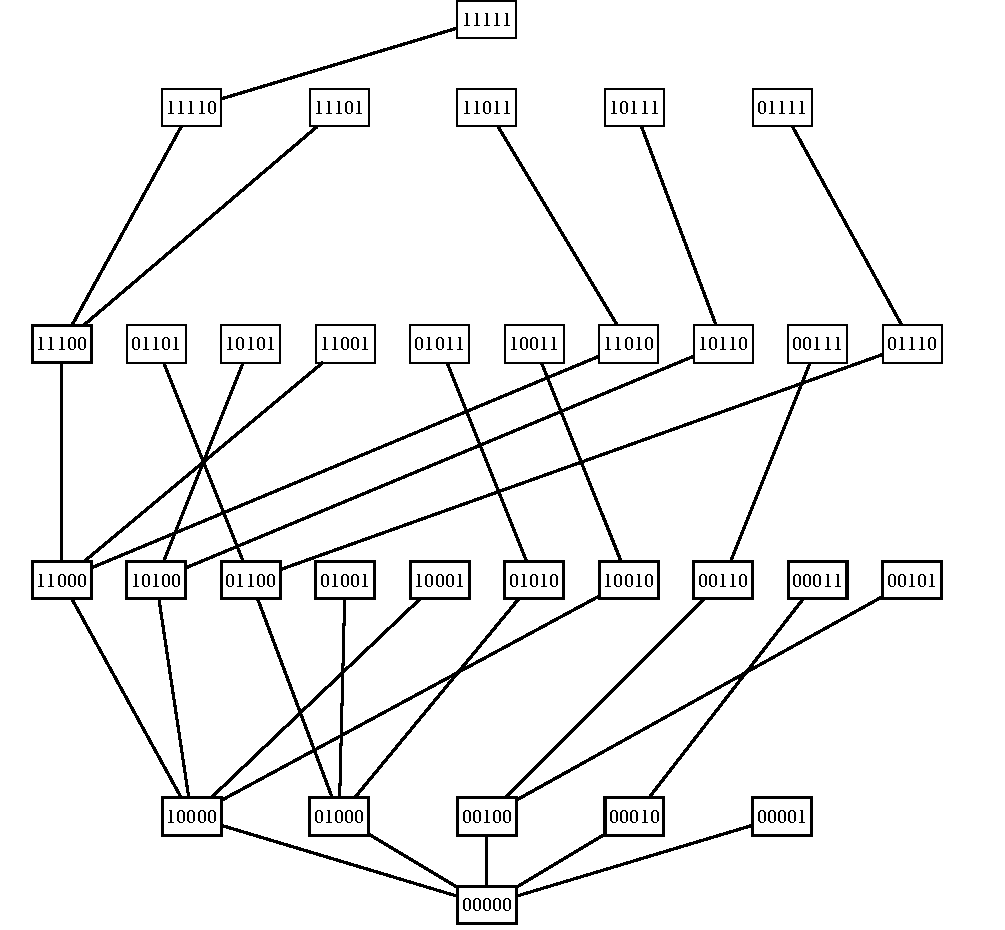
\includegraphics[clip=true]{pfs/ubb/ubb_tree.pdf}}
    \label{fig:ubb:tree} }
  \end{tabular}
    \caption{A figura ~\ref{fig:ubb:full} é o diagrama de Hasse do
    reticulado Booleano ($\powerset (S), \subseteq$) e a figura
    ~\ref{fig:ubb:tree} é uma árvore de busca definida pelo algoritmo
    \algname{UBB}.}
  \label{fig:pfs:ubb_tree} 
\end{figure}

A dinâmica do \algname{UBB} é simples. Aplica-se o lema 
~\ref{lemma:lower_forest} para percorrer o espaço de busca enquanto o 
custo dos subconjuntos visitados se mantém ou diminui; quando o custo 
aumenta, podemos podar a sub-árvore que se inicia no nó onde o custo 
cresce. Por exemplo, em uma instância do problema U-Curve com três 
características, se o custo do nó $Y = \{100\}$ é maior do que o custo 
de $\{000\}$ e, ao visitar $Y$, $X = \{011\}$ então podemos remover do 
espaço de busca todos os nós do intervalo $[100, 111]$.


\begin{algorithm}[!ht]
\textsc{U-Curve-Branch-and-Bound} $(S, c)$
\begin{algorithmic}[1]
    \State $\mathcal{M} \gets \mathsc{Branch} (S, \emptyset, c, c (\emptyset))$
    \Return $\{M \in \mathcal{M} : c(M) \text{é mínimo}\}$
\end{algorithmic}
\vspace{1em}

\textsc{Branch} $(X, Y, c, cost_Y)$
\begin{algorithmic}[1]
    \State $\mathcal{M} \gets \{Y\}$
    \While{$X \ne \emptyset$}
        \State remova um elemento $x$ de $X$
        \State $Y' \gets Y \cup \{y\}$
        \State $cost_{Y'} \gets c (Y')$
        \If {$cost_{Y'} \leq cost_Y$}
            \State $\mathcal{N} \gets \mathsc{Branch} (X, Y', c, cost_{Y'})$
            \State $\mathcal{M} \gets \mathcal{N} \cup \mathcal{M}$
        \EndIf
    \EndWhile
    \Return $\mathcal{M}$
\end{algorithmic}
\caption{Pseudo-código do algoritmo \algname{UBB}}
\end{algorithm}

Uma vez entendido como as podas acontecem, é fácil perceber que o 
\algname{UBB} precisa percorrer uma cadeia inteira (não há podas) quando
o custo nela não aumenta até o penúltimo nó da cadeia. Portanto, se a 
função de custo é, por exemplo, monótona não-crescente, então a condição
de poda nunca será verdadeira em qualquer cadeia do reticulado, logo 
todo o espaço de busca será visitado, como em uma busca exaustiva. Esta
é a maior limitação do algoritmo \algname{UBB} e foi para enfrentá-la 
que o algoritmo \algname{PFS} foi criado.

\subsection{O algoritmo \algname{Poset-Forest-Search}}
% - criação das duas árvores
% - percorrimento e poda
% - como manter as duas árvores representando o mesmo espaço de busca?
%   - regras de poda
%   - florestas
% - 
O algoritmo \algname{Poset-Forest-Search} (\algname{PFS}) é uma 
generalização do \algname{UBB} capaz de percorrer o espaço de busca em
duas direções, do menor para o maior elemento do reticulado 
(como o \algname{UBB}) e também do maior elemento para o menor. 
Para fazer isso, o \algname{PFS} inicia sua busca com duas árvores 
complementares, uma gerada por 
aplicações recursivas do lema ~\ref{lemma:lower_forest} e outra, que 
representa o reticulado Booleano dual ($\powerset (S), \supseteq$), 
gerada por aplicações recursivas do lema ~\ref{lemma:upper_forest}.

\begin{mylemma}
\label{lemma:upper_forest}
Sejam $X$ e $Y$ conjunto, $X$ não-vazio e $x_i$o $i$-ésimo 
elemento de $X$. Seja $X_0 \supseteq X_1 \supseteq \dots \supseteq 
X_{|X|}$ uma cadeia tal que $X_0 = X$, $X_{|X|} = \emptyset$ e $X_{i} 
\cup \{x_i\} = X_{i - 1}$ para todo $0 < i \leq |X|$. Vale que:
\begin{align*}
    \{ Y \cup X\} \cup \bigcup_{i = 1}^{|X|} \{(X - (W \cup {x_i})) \cup Y : W \in \powerset (X_i)\} = \{W \cup Y : W \in \powerset (X)\}.
\end{align*}
\end{mylemma} 

%TODO: demonstração

A figura ~\ref{fig:pfs:pfs_trees} mostra duas árvores do espaço de busca
geradas pelo algoritmo. Note que estas árvores permitem o percorrimento
do espaço de busca em duas direções. Observe também que na construção
da árvore que percorre o reticulado do conjunto menor para o maior 
(figura ~\ref{fig:pfs:lower}), o conjunto de nós alcançáveis por $Y$ é 
determinado pelo intervalo $[Y, X \cup Y]$, e na árvore dual (figura 
~\ref{fig:pfs:upper}), construída por aplicações recursivas do lema 
~\ref{lemma:upper_forest} o conjunto de nós alcançáveis por $Y$ é dado 
pela intervalo $[Y \setminus X, Y]$.

\begin{figure}[!ht]
  \centering 
  \begin{tabular}{c c}
    \subfigure[] {\scalebox{0.4}{
     \includegraphics[clip=true]{pfs/pfs/lower_tree.pdf}}
     \label{fig:pfs:lower} }
    & 
    \subfigure[] {\scalebox{.4}{
    \includegraphics[clip=true]{pfs/pfs/upper_tree.pdf}}
    \label{fig:pfs:upper} }
  \end{tabular}
    \caption{Exemplo de árvores do espaço de busca gerado pelo 
    algoritmo \algname{PFS}. A figura ~\ref{fig:pfs:lower} mostra a 
    árvore gerada por aplicações recursivas do lema 
    ~\ref{lemma:lower_forest} enquanto a figura ~\ref{fig:pfs:upper} 
    mostra a árvore gerada por aplicações recursivas do lema 
    ~\ref{lemma:upper_forest}.}
  \label{fig:pfs:pfs_trees}
\end{figure}

No algoritmo \algname{UBB} o controle do espaço de busca pode ser 
facilmente implementado, pois basta não inserir a sub-árvore podada na 
pilha de busca em profundidade. No \algname{PFS}, uma estratégia 
equivalente é capaz apenas de restringir nós da estrutura de dados que 
foi utilizada para o percorrimento de cadeias, ou seja, uma poda neste 
algoritmo implica na atualização das duas estruturas de dados que 
controlam o espaço de busca. Então, quando removemos um intervalo
de uma árvore, precisamos remover este mesmo intervalo da árvore dual; 
como resultado, a árvore dual se torna uma {\bf floresta}. Portanto, o
\algname{PFS} usa duas florestas para gerir o espaço de busca, uma
com caminhos de conjuntos menores para maiores, $\forest_A$ e outra 
dual, $\forest_B$. Um exemplo de atualização de árvore dual é
apresentado na figura ~\ref{fig:pfs:forest_prune}.

\begin{figure}[!ht]
  \centering 
  \begin{tabular}{c c}
    \subfigure[] {\scalebox{0.4}{
     \includegraphics[clip=true]{pfs/pfs/forest/lower_tree.pdf}}
     \label{fig:pfs:forest_pruneA} }
    & 
    \subfigure[] {\scalebox{.4}{
    \includegraphics[clip=true]{pfs/pfs/forest/upper_tree.pdf}}
    \label{fig:pfs:forest_pruneB} }
  \end{tabular}
    \caption{Exemplo de atualização de árvore após remoção de intervalo.
    Os nós em vermelho são removidos do espaço de busca enquanto os nós
    amarelos são raízes dos grafos. Removemos o intervalo 
    $[11100, 11111]$ da árvore da figura ~\ref{fig:pfs:forest_pruneA} e 
    ao remover este mesmo intervalo da árvore dual, o grafo perde a 
    raiz original $(11111)$ e ganha as três raízes em amarelo.}
    \label{fig:pfs:forest_prune}
\end{figure}

O \algname{PFS} inicia escolhendo arbitrariamente uma direção de 
percorrimento e uma raíz da floresta correspondente a direção escolhida.
O passo seguinte é a ramificação, que similar ao \algname{UBB} percorre 
uma cadeia da árvore escolhida enquanto o custo dos subconjuntos não 
cresce e não chegamos em uma folha da árvore. Ao fim da fase de 
ramificação, suponha que feita na floresta $\forest_A$ ($\forest_B$),
teremos um intervalo $[Y, X \cup Y]$ ($[Y \setminus X, Y]$) que precisa
ser removido da floresta dual. Esta atualização da floresta dual é 
feita de acordo com as seguintes regras.

\begin{mylemma}
\label{lemma:upper_update}
Sejam $T$ e $T'$ duas árvores tais que $T$ é complementar a $T'$. 
Eliminar de $T'$ os vértices contidos no intervalo $[Y, X \cup Y]$ é 
equivalente a remover de $T'$ todos os vértices do caminho $P$ de $T$ 
com extremos $Y$ e $X \cup Y$ e também todos os vértices de $T'$ 
contidos em intervalos $[Y, B]$ tais que $B$ contém propriamente $Y$ e 
$B$ é adjacente inferior a um vértice de $P$.
\end{mylemma}

\begin{mylemma}
\label{lemma:lower_update}
Sejam $T$ e $T'$ duas árvores tais que $T$ é complementar a $T'$. 
Eliminar de $T$ os vértices contidos no intervalo $[Y \setminus X, Y]$ 
é equivalente a eliminar de $T$ todos os vértices do caminho $P$ em $T$
com extremos $Y \setminus X$ e $Y$ e também todos os vértices de $T$
contidos em intervalos $[A, Y]$ tais que $A$ é contido propriamente em
$Y$ e $A$ é adjacente superior a um vértice de $P$.
\end{mylemma}

As demonstrações dos lemas ~\ref{lemma:upper_update} e 
~\ref{lemma:lower_update} estão disponíveis em Reis ~\cite{Rei12}.

O funcionamento do algoritmo deve seguir as seguintes regras:
\begin{enumerate}[a)]
    \item{\it Inicialização das florestas:} as florestas $\forest_A$ e 
        $\forest_B$ são iniciadas com as raízes $\emptyset$ e $S$ 
        respectivamente. \label{pfs:rule:a}
    \item{\it Representação de árvores:} para todo nó do espaço de busca 
        que não foi removido e não é raiz na floresta, a sub-árvore que
        se inicia neste nó está completa no espaço de buscas. Desta 
        forma, para representar a floresta precisamos apenas armazenar
        as raízes da floresta e suas adjacências, pois sabemos que cada
        vértice adjacente é raiz de uma subárvore completa. 
        \label{pfs:rule:b}
    \item{\it Gerenciamento das florestas:} durante a etapa de 
        ramificação, um vértice visitado é podado ou torna-se raiz na 
        floresta. Com isso, temos que todas arestas de um caminho 
        percorrido são removidas da floresta. \label{pfs:rule:c}
    \item{\it Condição de poda (dual):} no percorrimento de uma cadeia,
        se o nó $Y$ da floresta $\forest_A$ ($\forest_B$) tem custo 
        maior que o último nó visitado nesta cadeia, então removemos da
        floresta $\forest_A$ ($\forest_B$) a subárvore que
        começa em $Y$, $[Y, X \cup Y]$ ($[Y \setminus X, Y]$). Se um nó
        $Y$ visitado não tem conjuntos adjacentes no espaço de busca, 
        então $Y$ é removido do espaço de busca.
        \label{pfs:rule:d}
    \item{\it Atualização de floresta:} ao podar o intervalo 
        $[Y, X \cup Y]$ ($[Y \setminus X, Y]$) da floresta $\forest_A$
        ($\forest_B$), devemos remover os mesmos subconjuntos da outra
        floresta de acordo com o lema ~\ref{lemma:upper_update}
        (\ref{lemma:lower_update}). \label{pfs:rule:e}
\end{enumerate}


\subsection{Pseudo-código e detalhes de implementação do \algname{PFS}}
Apresentamos nesta seção um pseudo-código para o algoritmo e ao mesmo
tempo comentamos como algumas destas soluções foram implementadas por
Reis em \toolname{C++} no arcabouço \toolname{featsel}.

\subsubsection{Definição de árvores de busca}
Os algoritmos que descrevemos neste capítulo dependem da aplicação 
recursiva dos lemas ~\ref{lemma:lower_forest} e 
~\ref{lemma:upper_forest}, e para cada ordem de características $x_i$
escolhida na aplicação do lema obtemos uma árvore diferente para 
representar o espaço de busca (veja figura ~\ref{fig:pfs:tree_def}). A 
implementação de Reis possui uma enumeração sobre as características 
que nos permite fixar os resultados da aplicação recursiva destes lemas 
e também facilita o controle das árvores da floresta. Supomos então
que o conjunto de características $S$ é uma lista ordenada 
$\langle s_1, s_2, \dots, s_n \rangle$ e que é possível obter o índice 
de um elemento. Assim, sempre que fazemos a decomposição do espaço em 
uma árvore (com ambos lemas) escolhemos as variáveis do conjunto $X$ em
ordem crescente de índice.

\begin{figure}[!ht]
  \centering 
  \begin{tabular}{c c c}
    \subfigure[] {\scalebox{0.7}{
     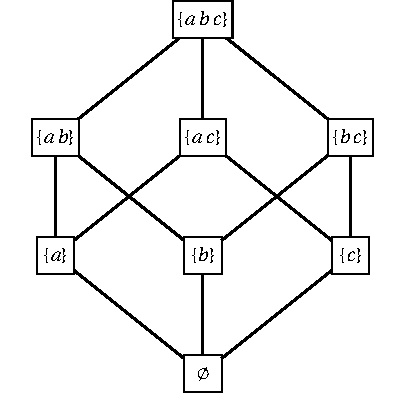
\includegraphics[clip=true]{pfs/feature_enum/original_lattice.pdf}}
     \label{fig:pfs:tree_def:A}}
    & 
    \subfigure[] {\scalebox{.7}{
     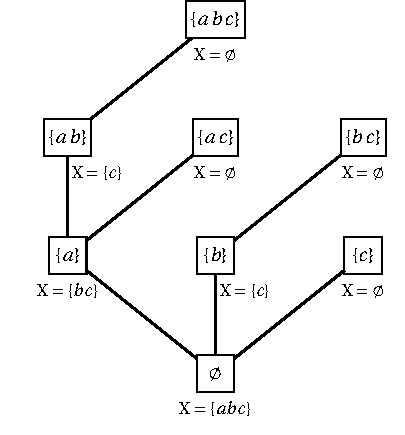
\includegraphics[clip=true]{pfs/feature_enum/treeA.pdf}}
    \label{fig:pfs:tree_def:B}}
    & 
    \subfigure[] {\scalebox{.7}{
     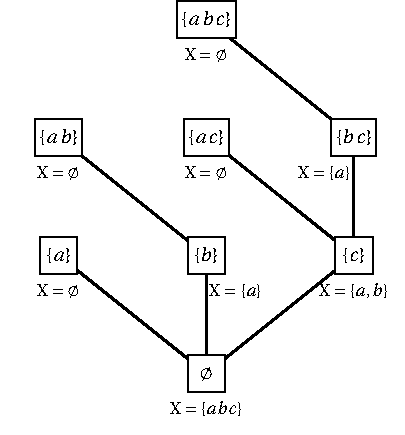
\includegraphics[clip=true]{pfs/feature_enum/treeB.pdf}}
    \label{fig:pfs:tree_def:C}}
  \end{tabular}
    \caption{Exemplos de aplicações recursivas do lema 
    ~\ref{lemma:lower_forest} no reticulado booleano da figura 
    ~\ref{fig:pfs:tree_def:A}. O conjunto $X$ indica para cada 
    subconjunto $Y$ qual é o conjunto de nós de sua sub-árvore: 
    exatamente os nós do intervalo $[Y, X \cup Y]$. Na figura 
    ~\ref{fig:pfs:tree_def:B} a decomposição elimina de $X$ os elementos
    na ordem $\langle a, b, c \rangle$ em todos os níveis de aplicação 
    do lema, enquanto na figura ~\ref{fig:pfs:tree_def:C} a ordem é 
    $\langle c, b, a \rangle$.}
    \label{fig:pfs:tree_def}
\end{figure}

\subsubsection{Estrutura de dados}
Vamos definir a estrutura de dados utilizada por Reis para representar
nós das florestas. Um nó $\pfsnode{N}$ é composto por quatro campos:
\begin{itemize}
    \item{\varname{vertex}:} armazena o conjunto de características que 
        o nó representa. 
    \item{\varname{adjacent}:} armazena um conjunto de características
        que determina a adjacência do nó. Um nó $\pfsnode{N}$ é 
        adjacente aos conjuntos de características 
        $\{\pfsnode{N}[\varname{vertex}] \cup \{x_i\} : x_i \in \pfsnode{N}[\varname{adjacent}]\}$.
    \item{\varname{leftmost}}: um inteiro que define, pelo esquema de
        numeração, o conjunto de características $X$ da decomposição
        em árvore do espaço de busca. Isto é, se
        $Y = \pfsnode{N}[\varname{vertex}]$ então o conjunto de nós da 
        sub-árvore com raiz $Y$ deve ser igual ao intervalo 
        $[Y, X \cup Y]$, se $\pfsnode{N}$ é da floresta $\forest_A$, ou
        igual ao intervalo $[Y \setminus X, Y]$ se $\pfsnode{N}$ é da 
        floresta $\forest_B$. Lembrando que assumimos uma ordem no 
        conjunto de características ($\langle s_1, s_2, \dots, 
        s_n\rangle$), $X$ é definido como 
            $X = \bigcup_{i = leftmost}^{n} s_i$.
    \item{$\varname{cost}$:} um número em ponto flutuante que armazena
        o custo de $\pfsnode{N}[\varname{vertex}]$.
\end{itemize}

Como descrevemos na seção anterior, uma das regras do algoritmo garante
que para representar as florestas precisamos apenas armazenar as raízes
das florestas e suas listas de adjacências. Desta maneira, as duas 
florestas $\forest_A$ e $\forest_B$ são representadas por conjuntos de
nós. Estes nós são armazenados na estrutura de \toolname{map} da 
linguagem \langname{C++}. 
\newpage
\subsubsection{Pseudo-código}
Vamos agora apresentar um pseudo-código do \algname{PFS} em uma 
abordagem que mostra primeiro o todo e depois cada parte.

Uma iteração qualquer do \algname{PFS} começa com a inicialização das 
florestas do espaço de busca. A floresta $\forest_A$, que permite 
percorrimentos de baixo para cima no reticulado, é inicializada com 
a raiz $\emptyset$ enquanto a floresta $\forest_B$, de percorrimentos
de cima para baixo, é inicializada com a raiz $S$. Assim que 
inicializadas as florestas, repetimos as etapas de escolha de direção
de percorrimento, ramificação e poda das florestas até que ambas 
estejam vazias. Note que não importa qual floresta devemos verificar
para terminar as iterações do algoritmo, já que ambas representam o 
mesmo espaço de busca, ou seja, quando uma floresta é vazia a outra 
também é.

\begin{algorithm}[H]
\textsc{Poset-Forest-Search} $(S, c)$
\begin{algorithmic}[1]
    \State $\mathcal{M} \gets \emptyset$
    \State $\pfsnode{T}[\varname{vertex}] \gets \emptyset$
    \State $\pfsnode{T'}[\varname{vertex}] \gets S$
    \State $\pfsnode{T}[\varname{cost}] \gets \pfsnode{T'}[\varname{cost}] \gets \infty$
    \State $\pfsnode{T}[\varname{adjacent}] \gets \pfsnode{T'}[\varname{adjacent}] \gets S$
    \State $\pfsnode{T}[\varname{leftmost}] \gets \pfsnode{T'}[\varname{leftmost}] \gets 1$
    \State $\forest_A \gets \{\pfsnode{T}\}$
    \State $\forest_B \gets \{\pfsnode{T'}\}$
    \While{$\forest_A \ne \emptyset$} \Comment{idêntico a $\forest_B \ne \emptyset$}
        \State $direction \gets \mathsc{Choose-Direction}$
        \If{$direction$}
            \State $\langle \mathcal{N}, \forest_A, \pfsnode{N} \rangle \gets \mathsc{Lower-Forest-Branch} (\forest_A, \forest_B, c)$
            \State $\forest_B \gets \mathsc{Upper-Forest-Prunning} (\forest_B, \pfsnode{N})$
        \Else
            \State $\langle \mathcal{N}, \forest_A, \pfsnode{N} \rangle \gets \mathsc{Upper-Forest-Branch} (\forest_A, \forest_B, c)$
            \State $\forest_A \gets \mathsc{Lower-Forest-Prunning} (\forest_A, \pfsnode{N})$
        \EndIf
        \State $\mathcal{M} \gets \mathcal{M} \cup \mathcal{N}$
    \EndWhile
    \Return $\{M \in \mathcal{M} : c(M) \text{é mínimo}\}$
\end{algorithmic}
\vspace{1em}
\caption{Pseudo-código do algoritmo \algname{PFS}}
\label{pfs:code:pfs:A}
\end{algorithm}

\newpage
A etapa de ramificação da floresta $\forest_A$ é feita pela função 
\textsc{Lower-Forest-Branch} e consiste no percorrimento, a partir de uma 
raiz $Y$, de uma cadeia de sua sub-árvore. Nesta etapa, para manter 
válida a regra ~\ref{pfs:rule:c} devemos remover todas as arestas do 
caminho percorrido e transformar todos os nós visitados e não podados em 
raízes da floresta. O percorrimento termina ao atingir um nó 
$\pfsnode{N}$ que é folha ou que possui custo maior do que seu 
precedente no caminho percorrido; então o intervalo 
$[\pfsnode{N}[\varname{vertex}], \pfsnode{N}[\varname{vertex}] \cup \pfsnode{N}[\varname{adjacent}]]$
deve ser removido da floresta $\forest_A$. Esta função retorna o nó 
$\pfsnode{N}$, a floresta $\forest_A$ atualizada, e o conjunto 
$\mathcal{M}$ de subconjuntos percorridos que são candidatos a mínimo.

\begin{algorithm}[H]
\textsc{Calc-Node-Cost} $(\forest, \pfsnode{N})$
\begin{algorithmic}[1]
\If{$\pfsnode{N}[\varname{cost}] = \infty$ e existe $\pfsnode{M} \in \forest$ tal que $\pfsnode{M}[\varname{vertex}] = \pfsnode{N}[\varname{vertex}]$ e $\pfsnode{M}[\varname{cost}] \ne \infty$}
    \Return $\pfsnode{M}[\varname{cost}]$
\Else
    \Return $c(\pfsnode{R}[\varname{vertex}])$
\EndIf
\end{algorithmic}
\end{algorithm}

\begin{algorithm}[ht]
\textsc{Lower-Forest-Branch} $(\forest_A, \forest_B, c)$
\begin{algorithmic}[1]
    \State $\mathcal{M} \gets \emptyset$
    \State remova um nó $\pfsnode{R}$ de $\forest_A$
    \State $\pfsnode{R}[\varname{cost}] \gets \mathsc{Calc-Node-Cost}(\forest_B, \pfsnode{R})$
    \State $\pfsnode{M} \gets \pfsnode{N} \gets \pfsnode{R}$
    \While{$\pfsnode{N}[\varname{cost}] \leq \pfsnode{M}[\varname{cost}]$ e $\pfsnode{N}[\varname{adjacent}] \ne \emptyset$}
        \State $\pfsnode{M} \gets \pfsnode{N}$
        \State remova um elemento de $s_i$ de $\pfsnode{M}[\varname{adjacent}]$
        \State $\forest_A \gets \forest_A \cup \{\pfsnode{M}\}$
        \State crie o nó $\pfsnode{N}$
        \State $\pfsnode{N}[\varname{vertex}] \gets \pfsnode{M}[\varname{vertex}] \cup \{s_i\}$
        \State $\pfsnode{N}[\varname{leftmost}] \gets i$
        \State $\pfsnode{N}[\varname{adjacent}] \gets \bigcup_{i=\pfsnode{N}[\varname{leftmost}]}^{n} s_i$
        \State $\pfsnode{N}[\varname{cost}] \gets \mathsc{Calc-Node-Cost} (\forest_B, \pfsnode{N})$
        \State $\mathcal{M} \gets \mathcal{M} \cup \{\pfsnode{N}\}$
    \EndWhile
    \Return $\langle \mathcal{M}, \forest_A, \pfsnode{N}\rangle$
\end{algorithmic}
\caption{Continuação do pseudo-código ~\ref{pfs:code:pfs:A}, com a função
que faz o percorrimento da floresta $\forest_A$.}
\label{pfs:code:pfs:B}
\end{algorithm}


A ramificação dual, da floresta $\forest_B$ é feita pela função 
\textsc{Upper-Forest-Branch} e é similar a função 
\textsc{Lower-Forest-Branch} ao percorrer uma cadeia da floresta de 
conjuntos maiores para conjuntos menores. A ramificação termina ao 
encontrar um nó $\pfsnode{N}$ que é folha da floresta ou tem custo maior
que seu precedente no caminho; então o intervalo 
$[\pfsnode{N}[\varname{vertex}] \setminus \pfsnode{N}[\varname{adjacent}], \pfsnode{N}[\varname{vertex}]]$
deve ser removido da floresta $\forest_B$ e todos os nós visitados, 
menos $\pfsnode{N}$ tornam-se raízes. Esta função retorna o nó
$\pfsnode{N}$, a floresta $\forest_B$ atualizada e o conjunto 
$\mathcal{M}$ de subconjuntos percorridos que são candidatos a mínimo.

\newpage
A atualização da floresta $\forest_B$ após o percorrimento e poda da
floresta $\forest_A$ é feito pela função \textsc{Upper-Forest-Prunning}.
Esta função recebe um nó $\pfsnode{N}$ e deve remover os nós de 
$\forest_B$ de acordo com a regra ~\ref{pfs:rule:e}. Para fazer isto, 
percorremos o caminho $P$ que liga os nós de subconjuntos 
$\pfsnode{N}[\varname{vertex}]$ e $\pfsnode{N}[\varname{vertex}] \cup 
\pfsnode{N}[\varname{adjacent}]$ na floresta $\forest_B$, removendo cada
um dos nós deste caminho (se existirem) e chamando a função 
\textsc{Search-Lower-Children} para verificar se os filhos destes nós
devem ser podados ou não. Ao fim do caminho chamamos a função 
\textsc{Search-Upper-Root} para achar, na floresta $\forest_B$, a raiz
que alcança este caminho; fazemos isto para atualizar a adjacência desta 
raiz e garantir que uma ramificação não vai inserir os nós removidos. 
Esta função devolve a floresta $\forest_B$ atualizada.

\begin{algorithm}[H]
    \textsc{Get-Node} ($\forest, N$)
    \begin{algorithmic}[1]
        \If{existe $\pfsnode{N} \in \forest$ tal que $\pfsnode{N}[\varname{vertex}] = N$}
            \Return $\pfsnode{N}$
        \Else
            \Return $NIL$
        \EndIf
    \end{algorithmic}
    \vspace{1em}
    \textsc{Uppper-Forest-Prunning} ($\forest_A, \forest_B, \pfsnode{N}$)
    \begin{algorithmic}[1]
        \State $M \gets \pfsnode{N}[\varname{vertex}]$
        \While{$\pfsnode{N}[\varname{adjacent}] \ne \emptyset$}
            \State $\pfsnode{M} \gets \mathsc{Get-Node} (\forest_B, M)$
            \If{$\pfsnode{M} \ne NIL$}
                \State remova $\pfsnode{M}$ de $\forest_B$
            \EndIf
            \State $\forest_B \gets \mathsc{Search-Lower-Children} (\forest_B, \pfsnode{M}, M, \pfsnode{N}[\varname{vertex}])$
            \State remova o elemento $s_i$ de $\pfsnode{N}[\varname{adjacent}]$ com maior $i$
            \State $M \gets M \cup \{s_i\}$
        \EndWhile
        \State $\pfsnode{M} \gets \mathsc{Get-Node} (\forest_B, M)$
        \If{$\pfsnode{M} = NIL$}
            \State $\mathsc{Search-Upper-Root} (\forest_B, M)$
        \Else
            \State remova $\pfsnode{M}$ de $\forest_B$
        \EndIf
        \State $\forest_B \gets \mathsc{Search-Lower-Children} (\forest_B, \pfsnode{M}, M, \pfsnode{N}[\varname{vertex}])$
        \Return $\forest_B$
    \end{algorithmic}
    \caption{Continuação do pseudo-código ~\ref{pfs:code:pfs:B}, com a
    função que faz a atualização da floresta $\forest_B$ depois de um 
    percorrimento em $\forest_A$.}
    \label{pfs:code:pfs:C}
\end{algorithm}



A atualização dual, da floresta $\forest_A$, após o percorrimento e 
poda da floresta $\forest_B$ é feito pela função 
\textsc{Lower-Forest-Pruning} e seu funcionamento é parecido com o de
\textsc{Upper-Forest-Pruning}. O caminho $P$ de $\forest_A$ que deve 
ser removido tem as pontas 
$\pfsnode{N}[\varname{vertex}] \setminus \pfsnode{N}[\varname{adjacent}]$
e $\pfsnode{N}[\varname{vertex}]$, e a função 
\textsc{Search-Upper-Children} é chamada para verificar se os filhos 
destes nós devem ser podados ou não. Ao fim do caminho chamamos a função 
\textsc{Search-Lower-Root} para achar, na floresta $\forest_A$, a raiz
que alcança este caminho. Esta função devolve a floresta $\forest_A$
atualizada.

\newpage
A função \textsc{Search-Lower-Children} é chamada para cada nó $M$ do 
caminho $P$, como descrito no lema ~\ref{lemma:upper_update}. Esta 
função verifica para todos os filhos $B$ de $M$ se $B$ contém 
propriamente o conjunto $\pfsnode{N}[\varname{vertex}]$; se contém, o 
nó de subconjunto $B$ deve ser removido da floresta, caso 
contrário, um nó que representa este conjunto deve ser tornar raiz da 
floresta, pois o pai de $B$ está sendo removido da floresta e isto 
significa que não haverá raiz que alcance $B$. Esta função
devolve a floresta $\forest_B$ atualizada.

\begin{algorithm}[H]
\textsc{Search-Lower-Children} $(\forest_B, \pfsnode{M}, M, Y)$
\begin{algorithmic}[1]
    \State $i \gets n$
    \While{$i \geq 1$ e $s_i \in M$}
        \State $B \gets M \setminus \{s_i\}$
        \If{$B \supseteq Y$}
            \State $\pfsnode{B} \gets \mathsc{Get-Node} (\forest_B, M)$
            \If{$\pfsnode{B} \ne NIL$}
                \State remova $\pfsnode{B}$ de $\forest_B$
            \EndIf
        \Else
            \State crie o nó $\pfsnode{B}$
            \State $\pfsnode{B}[\varname{vertex}] \gets B$
            \State $\pfsnode{B}[\varname{leftmost}] \gets i + 1$
            \State $\pfsnode{B}[\varname{adjacent}] \gets \bigcup_{i=\pfsnode{B}[\varname{leftmost}]}^{n} s_i$
            \State $\pfsnode{B}[\varname{cost}] \gets \infty$
            \State $\forest_B \gets \forest_B \cup \{\pfsnode{B}\}$ 
        \EndIf
        \State $i \gets i - 1$
        \Return $\forest_B$
    \EndWhile
\end{algorithmic}
\caption{Continuação do pseudo-código ~\ref{pfs:code:pfs:C}}
\label{pfs:code:pfs:D}
\end{algorithm}


\textsc{Search-Upper-Children} é a função dual de 
\textsc{Search-Lower-Children} e faz um procedimento similar, para 
cada nó $\pfsnode{M}$ do caminho $P$, como descrito no lema 
~\ref{lemma:lower_update}. Esta função verifica para todos os filhos $A$
de $M$ se $A$ é contido propriamente pelo conjunto 
$\pfsnode{N}[\varname{vertex}]$; se é, o nó de subconjunto $A$ deve ser 
removido da floresta, caso contrário, o um nó que representa o conjunto 
$A$ deve se tornar raiz da floresta. Esta função devolve a floresta 
$\forest_A$ atualizada.


A função \textsc{Search-Upper-Root} recebe um subconjunto $M$ e a 
floresta $\forest_B$. O objetivo desta função é remover arestas da 
floresta que podem levar ao conjunto $M$. Para isto, a função deve 
percorrer um caminho de $M$ até uma raiz da floresta (de conjuntos 
menores para maiores), e esta raiz deve ter sua lista de adjacência 
atualizada, removendo a aresta que a comunica com $M$. Para garantir que 
removemos todas as arestas, devemos criar raízes para todos nós deste 
caminho mas sem a adjacência que os comunica com $M$. O funcionamento de 
\textsc{Search-Lower-Root} é similar, mas deve ocorrer em outra direção
(de conjuntos maiores para menores).

\begin{algorithm}[H]
\textsc{Search-Upper-Root} $(\forest_B, M)$
\begin{algorithmic}[1]
    \State $i \gets n$
    \While{$i \geq 1$ e $s_i \in M$}
        \State $i \gets i - 1$
    \EndWhile
    \While{$i \geq 1$}
        \State $m \gets s_i$
        \State $M \gets M \cup \{m\}$
        \State $\pfsnode{M} \gets \mathsc{Get-Node} (\forest_B, M)$
        \If{$\pfsnode{M} \ne NIL$}
            \State $\pfsnode{M}[\varname{adjacent}] \gets \pfsnode{M}[\varname{adjacent}] \setminus \{m\} $
            \State $i \gets 0$
        \Else
            \State crie o nó $\pfsnode{M}$
            \While{$i \geq 1$ e $s_i \in M$}
                \State $i \gets i - 1$
            \EndWhile
            \State $\pfsnode{M}[\varname{leftmost}] \gets i + 1$
            \State $\pfsnode{M}[\varname{adjacent}] \gets \cup_{j = \pfsnode{M}[\varname{leftmost}]}^{n} \{s_j\} \setminus \{m\} $
            \State $\pfsnode{M}[\varname{cost}] \gets \infty$
            \State adicione $\pfsnode{M}$ em $\forest_B$
        \EndIf
        \Return $\forest_B$
    \EndWhile
\end{algorithmic}
\end{algorithm}

\section{Melhoramentos na escolha de raiz}
% - começar falando sobre o problema... 
%   a escolha era feita de maneira arbitrária. Estrutura de map guardava
%   as raízes e escolhia-se o primeiro elemento do map, que de acordo com blabla
%   será o menor elemento lexicograficamente ou o maior 
% - por que mudar isso pode melhorar? Porque o critério é arbitrário
% - aleatória: talvez traga melhoras se a abordagem anterior escolhesse 
%   raízes ruins
% - "leftmost": estamos priorizando percorrer as maiores árvores, em 
%   tese
Reis utilizou a estrutura de \toolname{map} para armazenar as raízes das 
florestas do espaço de busca. Como chave das raízes, utiliza-se a 
\toolname{string} que representa o vetor característico da raiz. A 
estrutura de \toolname{map} em \langname{C++}, geralmente implementada
com árvores binárias de busca, mantém os elementos ordenados pelo valor
de sua chave, portanto as raízes são armazenadas de maneira ordenada
lexicograficamente.

A estratégia adotada por Reis na escolha de uma raiz da floresta 
consiste em escolher de maneira equiprovável o primeiro ou o último 
elemento do \toolname{map} de raízes. Esta estratégia é aleatória e é 
viesada pois tende a escolher os primeiros ou últimos elementos de uma 
ordenação. Como esta estratégia de ordenação é arbitrária e não existe 
aparente fundamentação lógica que a justifique, acreditamos que novas 
estratégias de escolhas de raízes podem trazer melhores resultados ao 
algoritmo \algname{PFS}.

\subsection{Escolha equiprovável}
A primeira estratégia que testamos foi uma escolha também aleatória, mas
com uma distribuição de probabilidade de escolhas igual para cada raíz
da floresta. Como a estratégia de Reis é viesada, julgamos necessário
investigar se este viés não leva o algoritmo a fazer ramificações ou 
podas ruins, que comprometessem o tempo de execução do algoritmo. Se
o tempo de execução com a nova estratégia é menor, então confirmamos
esta hipótese.

Para implementar esta nova escolha, utilizamos a mesma estrutura de 
dados 

\section{Melhoramentos no controle de raízes}
% - quando o número de raízes é muito grande map é uma estrutura mais 
%   cara para consultas e inserções, enquanto nas ROBDDs essa operação é 
%   mais barata(?)
%     - explicar ROBDDs
% - uso de ROBDD
%   com raíz aleatória e com raíz leftmost

\section{Paralelização do código}
% utilizando a biblioteca OpenMP
% simplificação: paralelizamos iterações do código uma a uma
% complicado: as coisas são intrínsecas
%   -> o que é melhor: 
